\documentclass[12pt,fleqn]{article}\usepackage{../common}
\begin{document}
Dinamik Programlama

Dinamik programlamanin (DP) temelinde ardi ardina verilen kararlarin
bulunmasi / hesaplanmasi fikri vardir; ilgilendigi problemler her verilen
kararin diger karar seceneklerini ortaya cikardigi turden problemlerdir, ve
her seferinde bu seceneklerin arasindan bir tanesi secilmelidir. Amac en
iyi karar zincirini bulmaktir. Metot olarak kullanilanlar kismen ``acgozlu
algoritmalar (greedy algorithms)'' olarak bilinen algoritmalarin yaptigina
benzer fakat acgozlu algoritmalar, mesela en kisa yolu bulmaya ugrasirken,
gezilen dugumlerde sadece ``o an icin'' en iyi secimi yapar. Bu tur secim
nihai sonuc goze alindigi zamanen iyi sonucu vermeyebilir; Mesela alttaki
grafige bakarsak,

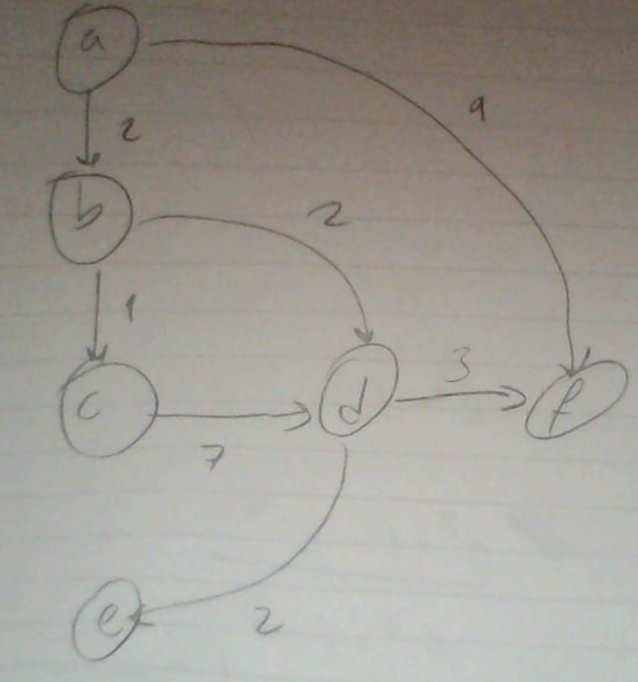
\includegraphics[height=6cm]{dp1.jpg}

diyelim ki \verb!a! noktasindan \verb!f! noktasina en kisa yoldan ulasmaya
calisiyoruz - acgozlu algoritma \verb!a,b,c,d! uzerinden gidis yapardi
cunku her an, sadece o an icin en iyi olani secerdi. Fakat nihai sonuca
bakarsak secilen yolun en kisa yol olmadigini goruruz. En iyi yol
\verb!a,b,d! uzerinden giden yoldur.

Gosterilen cizit / ag yapisi (graph) yonlu ve �evrimsiz (directed, acyclic
graph -DAG-) diye bilinen bir yapidir. Tipik kisa yol problemleri bu
yapilar uzerinde calisirlar.

DP problemleri ozellikle bir problemi alt problemlere bolebildigimiz zaman
faydalidirlar, ve bu alt problemler tekrar tekrar hesaplaniyorlarsa da bu
daha iyidir, cunku DP o alt problemleri onbellekleyerek tekrar
hesaplanmadan geri getirilmelerini saglayabilir. 

Mesela ustteki en kisa yol problemini DP ile cozelim.

Once bazi teorik, mantiksal konular: tumevarimsal olarak dusunelim. Diyelim
ki ustteki DAG'de $a,f$ arasindaki en kisa yolu kesinlikle
``biliyoruz''. Ve yine diyelim ki bu yol uzerinde / bir ara nokta $x$
noktasi var. O zaman, $a,x$, ve $x,f$ arasindaki yollar da tanim itibariyle
en kisadir. Ispatlayalim: eger mesela $x,f$ arasindaki en kisa yol
bildigimizden {\em baska} olsaydi, o zaman eldekini atip o yolu kullaniyor
olurduk (en kisa oldugunu kesin biliyoruz ya), ve bu sefer o alternatif en
kisa olurdu. Fakat ilk basta en kisa yolu bildigimiz faraziyesi ile
basladik. Bir celiski elde ettik, demek ki ara noktanin kisaligi dogrudur
$\square$

Bu ispattan hareketle kisa yolu tek numerik bir deger olarak hesaplamaya
ugrasabiliriz. 

Oyle bir fonksiyon $d(v)$ olsun ki herhangi bir $v$ nodu icin o nod'dan
bitis noktasina olan en kisa uzakligi kesin biliyor olsun (dikkat, bu
hesabin nasil olacagini dusunmuyoruz simdilik, sadece olabilecegini, olmus
oldugunu farz ediyoruz). Cogu tumevarimsal tasarimda oldugu gibi hesabin
kendisinin ozyinelilik (recursive) cagri zincirinin mekanigi icinde
halolmasini amacliyoruz. Dogru olan bir ifadeyi dusunuyoruz oncelikle, ve
hesabin kendisini surekli bir sonraki noktaya erteliyoruz. 

Devam edelim: $u,v$ arasindaki parca mesafeler $w(u,v)$'dir. Simdi, eger
bir ara nokta $u$'ya gelmissek -yine tumevarimsal olarak dusunmeye devam
ediyoruz- bu noktanin her komsusu $w$ icin $d(w)$'yi ``bildigimize'' gore,
en kisa yol icin tek yapmamiz gereken her secim aninda en minimal $w(u,v) +
d(v)$'yi 
$u$'nun uzakligi olarak almaktir.

Veri yapisi olarak DAG'i alttaki gibi gosterelim,

\begin{minted}[fontsize=\footnotesize]{python}
DAG = {
    'a': {'b':2, 'f': 9},
    'b': {'d':2, 'c':1, 'f': 6},
    'c': {'d':7},
    'd': {'e':2, 'f': 3},
    'e': {'f':4},
    'f': {}
}
\end{minted}

Boylece $w(u,v)$ basit bir Python sozluk (dictionary) erisimi haline
geliyor, mesela \verb!a,b! arasi parca mesafe icin 

\begin{minted}[fontsize=\footnotesize]{python}
print DAG['a']['b']
\end{minted}

\begin{verbatim}
2
\end{verbatim}

En kisa yolu bulacak program

\begin{minted}[fontsize=\footnotesize]{python}
from functools import wraps

def memo(func):
    cache = {}                                  
    @wraps(func)                                
    def wrap(*args):                            
        if args not in cache:
            print 'onbellekte yok -', args[0]
            cache[args] = func(*args)
        else: print 'onbellekte var -', args[0]
        return cache[args]                      
    return wrap 

def rec_dag_sp(W, s, t): 
    @memo                                    
    def d(u):
        print 'Dugum:' + u[0]
        if u == t:  print 'Son nokta t, geri donus'; return 0  
        min_dist = min(W[u][v]+d(v) for v in W[u])  
        print 'Geri donus,',u,'uzerindeyiz, mesafe=',min_dist
        return min_dist
    return d(s)                                 

dist = rec_dag_sp(DAG, 'a', 'f')
print 'toplam mesafe=', dist
\end{minted}

\begin{verbatim}
onbellekte yok - a
Dugum:a
onbellekte yok - b
Dugum:b
onbellekte yok - c
Dugum:c
onbellekte yok - d
Dugum:d
onbellekte yok - e
Dugum:e
onbellekte yok - f
Dugum:f
Son nokta t, geri donus
Geri donus, e uzerindeyiz, mesafe= 4
onbellekte var - f
Geri donus, d uzerindeyiz, mesafe= 3
Geri donus, c uzerindeyiz, mesafe= 10
onbellekte var - d
onbellekte var - f
Geri donus, b uzerindeyiz, mesafe= 5
onbellekte var - f
Geri donus, a uzerindeyiz, mesafe= 7
toplam mesafe= 7
\end{verbatim}

Simdi cagri mekaniginin hakikaten nasil isledigini gorelim. Not: Onbellek
kodlamasi dekorator kullaniyor, dekoratorler hakkinda bir yazi icin [2]'ye
bakabilirsiniz.

Baslangic $u$, oradan, minimum secerken, surekli $d()$ cagrisi yapiyoruz,
yani $d()$ kendini cagiriyor. Cagrinin geri donmesinin tek yolu son noktaya
erismek. Bu ne demektir? Programimiz daha hesap yapmadan ``derinligine bir
dalis'' yapiyor. Son noktalara gelene kadar ozyineli cagrilari ardi ardina
uyguluyor, esas hesaplari geri donus sirasinda yapiyor. Bu nasil ise
yariyor? Ayrica onbelleklemenin hakikaten isleyip islemedigini nasil
bilecegiz?  Ya da onbellekteki bir degerin hep en iyisi oldugunu nereden
bilecegim? 

Bu arada, boyle bir yaklasimda, onbellek degeri bir kez set edildi mi,
hic degistirmeye gerek yok.

Nokta \verb!d!'ye bakalim. Bu noktanin mesafesi (yani son nokta \verb!f!'ye
uzakligi) kararlastirilirken algoritma \verb!d!'nin her komsusuna
bakacaktir, bunu \verb!for v in W[u])! ile yapacaktir. Her komsu icin
\verb!f!'ye gelene kadar o yol derinligine takip edilecektir.  Mesela
ustteki ciktida goruyoruz ki \verb!d! sonrasi iki komsu \verb!e,f! icin
once \verb!d-f! ve \verb!d-e-f! gidisi yapilmistir (amac hep o son noktaya
ulasmak, unutmayalim). 'Komsulara bakma ve aralarindan en azi secme''
mantigi tum bu yollar denenene kadar bekleyecektir, ancak hepsi bittikten
sonra iclerinden bir minimum sececektir.

Iste simdi niye her dugumdeki minimum hesabinin en iyisi oldugunu
anliyoruz, cunku o noktadan nihai noktaya varis icin tum alternatifler
deneniyor. O derine dalisin sonuclari arasindan bir tanesi
seciliyor. Onbellekteki deger bu sebeple bir kez set ediliyor, ve hic
degismiyor. Tabii ki onbellekteki deger tekrar tekrar kullanilabiliyor,
mesela \verb!c!  icin bir \verb!d! uzakligi gerektiginde bu onbellekten
servis edilecektir.

Ve her dugumdaki minimum hesabi en iyiyse, bu hesaplari kullanan baslangica
yakin noktalarin hesabi da dogal olarak en iyisi (kisasi) olacaktir. Basta
tumevarimsal olarak belirttigimizin tekrar ifade edilmesidir bu. 

Kisa Yol Tarifini Bulmak

Mesafe hesabi iste boyle yapiliyor... Peki en kisa yolun kendisini nasil
biliriz? Yani once suraya, sonra suraya git turunden yol tarifi bilgisi
nasil hesaplanir? Aslinda komsular arasindaki en kisa mesafeyi secme
problemi, o komsular icinden hangisinin o en mesafeyi sagladigini hatirlama
problemine oldukca benziyor. Yani, her dugum uzerindeyken ve komsular
arasindan en kisa mesafeyi secerken, o mesafenin ``hangi komsudan''
geldigini hatirlamak ve bunu bir yerlere kaydetmek yeterli. Her dugum icin,
son noktaya olan en kisa mesafe degismedigine gore, ``o mesafe bilgisinin
geldigi komsunun hangisi oldugu'' bilgisi de degismeyecektir. Ve her nokta
icin o ``ebeveyn komsu'' bilindigi zaman hersey isleyip bittikten sonra en
kisa yol tarifi icin eldeki kayda bakariz, ve baslangic noktasi
\verb!a!'dan baslayarak ziplaya ziplaya o ebeveyn zinciri ile sona kadar
geliriz. Bu degisiklikleri ekleyince kod su hale gelir,


\begin{minted}[fontsize=\footnotesize]{python}
parent = {}

def rec_dag_sp2(W, s, t):                       
    @memo                                      
    def d(u):                                  
        if u == t: return 0                    
        distances = [W[u][v]+d(v) for v in W[u]]
        min_dist = min(distances)
        parent[u] = list(W[u])[np.argmin(distances)]
        print 'Geri donus,',u,'uzerindeyiz, mesafe=',min_dist
        return min_dist
    return d(s)                                

print rec_dag_sp2(DAG, 'a', 'f')

print 'ebeveynler', parent
\end{minted}

\begin{verbatim}
onbellekte yok - a
onbellekte yok - b
onbellekte yok - c
onbellekte yok - d
onbellekte yok - e
onbellekte yok - f
Geri donus, e uzerindeyiz, mesafe= 4
onbellekte var - f
Geri donus, d uzerindeyiz, mesafe= 3
Geri donus, c uzerindeyiz, mesafe= 10
onbellekte var - d
onbellekte var - f
Geri donus, b uzerindeyiz, mesafe= 5
onbellekte var - f
Geri donus, a uzerindeyiz, mesafe= 7
7
ebeveynler {'a': 'b', 'c': 'd', 'b': 'd', 'e': 'f', 'd': 'f'}
\end{verbatim}

Not: \verb!argmin! bir liste icindeki en minimal degerin indisini verir. 

Iste sonuc. Baslangic \verb!a!, onun ebeveyni \verb!b!. \verb!b!'ye
bakiyoruz, onunki \verb!d!. Oradan \verb!f!'ye atliyoruz, ve sonuca erismis
oluyoruz, en kisa yol \verb!a-b-d-f!. 

Analiz

Acgozlu yaklasimdan bu yaklasimin farkini simdi daha iyi gorebiliriz,
acgozlu teknik her dugumde en azi bizzat takip eder, ve kisayol hesabi,
mesafe hesabi hep bu takip eylemi sirasin o anda yapilir, elde bir toplam
vardir ve ona eklenir, vs. Bu yaklasim daha hangi yolu sectigi, sonradan,
birkac adim sonrasinda hicbir secimle ilgilenmez. Dinamik Programlama ise
takip etme eylemi ile hesap eylemini birbirinden ayirir, ve tumevarimsal
bir tanimdan yola cikarak, hep en kisa, en optimali bulmayi basarir.

DP algoritmasinin karmasikligi, $M$ tane baglanti (edges) ve $N$ tane dugum
icin $O(N + M)$'dir. Yani cozum lineer zamandadir! Alt problemleri tekrar
tekrar cozuyoruz evet, ve \verb!@memo! ibaresini koddan cikartsaydik
algoritmamizin ustel (exponential) zamanda isledigini gorurduk, ki bu cok
kotudur. Fakat cozulen alt problemleri bir daha cozmeyip sonuclarini
onbellekten aldigimiz icin algoritma son derece hizli isliyor.

Kaynaklar

[1] Hetland, M., L., {\em Python Algorithms}, 8. Bolum

[2] \url{http://sayilarvekuramlar.blogspot.de/2013/07/onbelleklemeyi-dekorator-ile-yapmak.html}

\end{document}
